\documentclass[12pt,a4paper]{article}
\usepackage[utf8]{inputenc}
\usepackage{geometry}
\usepackage{graphicx}
\usepackage{amsmath}
\usepackage{hyperref}
\usepackage{lipsum}
\usepackage{float}

% Page layout
\geometry{top=1in, bottom=1in, left=1in, right=1in}

\begin{document}

% Title
\begin{titlepage}
    \centering
    {\Large\textbf{Deep Learning \\ Danger Spot for Pedestrians}\par} % Judul
    \vspace{2cm} % Jarak antara judul dan logo
    
\includegraphics[width=0.5\linewidth]{assets/Logo-Resmi-Unhas-1.png}\par % Logo
    \vspace{2cm} % Jarak antara logo dan nama
    {\large
    Sakinah Nurusyifa (H071221049)\\ 
    Kevin Al Gazali (H071221060)\\ 
    A M Fauzan Baihaqi T (H071221088)\par}
    \vspace{1cm} % Jarak antara nama dan tanggal
     % Informasi universitas dan tanggal
    \textbf{PROGRAM STUDI SISTEM INFORMASI}\\
    \textbf{FAKULTAS MATEMATIKA DAN ILMU PENGETAHUAN ALAM}\\
    \textbf{UNIVERSITAS HASANUDDIN}\\[0.5cm]
    {\large\today\par} % Tanggal
\end{titlepage}

\tableofcontents
\newpage

% 1. Introduction
\section{Introduction}
Keselamatan pejalan kaki di sekitar kawasan kampus Universitas Hasanuddin (Unhas) Tamalanrea menjadi isu yang cukup penting, namun sering kali terabaikan. Kampus Unhas Tamalanrea merupakan area dengan tingkat mobilitas yang tinggi, yang melibatkan mahasiswa, dosen, staf, serta masyarakat umum. Aktivitas sehari-hari di kawasan ini meliputi perjalanan ke kelas, keperluan administratif, serta sekadar melintas menuju area lain. Sayangnya, meskipun memiliki tingkat keramaian yang tinggi, banyak titik di sekitar kampus yang belum dilengkapi dengan fasilitas yang memadai untuk melindungi pejalan kaki. Hal ini menciptakan potensi bahaya yang besar, terutama bagi pejalan kaki yang berbagi ruang dengan kendaraan bermotor.

Meskipun tingkat mobilitas di sekitar kampus Unhas Tamalanrea sangat tinggi, keselamatan pejalan kaki sering kali tidak mendapatkan perhatian yang cukup. Banyak titik di kawasan tersebut yang tidak dilengkapi dengan fasilitas yang memadai untuk melindungi pejalan kaki, seperti trotoar yang layak. Kondisi ini meningkatkan risiko kecelakaan, baik yang melibatkan pejalan kaki maupun pengguna kendaraan bermotor. Perlu adanya pemetaan dan analisis mengenai titik-titik berbahaya yang dapat mengancam keselamatan pejalan kaki di area ini.

Tujuan dari penelitian ini adalah untuk menyediakan kumpulan data yang terdiri dari gambar-gambar spot berbahaya yang dapat membahayakan keselamatan pejalan kaki di dalam kampus Unhas Tamalanrea. Dataset ini akan berfokus pada pengambilan gambar secara langsung dari area-area yang memiliki kondisi infrastruktur yang tidak aman, seperti lantai yang pecah, sudut lantai yang tajam, dan lubang tanpa pembatas. Dengan adanya kumpulan gambar ini, pihak kampus dapat dengan mudah mengidentifikasi lokasi-lokasi yang memerlukan perhatian dan perbaikan. Selain itu, dataset ini juga diharapkan dapat digunakan sebagai referensi visual dalam perencanaan dan pengambilan keputusan terkait perbaikan infrastruktur di lingkungan kampus, guna menciptakan lingkungan yang lebih aman dan nyaman bagi seluruh pengguna fasilitas kampus. Melalui penyediaan data ini, penelitian ini bertujuan untuk membantu pihak kampus dalam mengimplementasikan langkah-langkah preventif yang diperlukan untuk meningkatkan keselamatan pejalan kaki di area kampus.

% 2. Related Works
\newpage
\section{Related Works}
Keselamatan pejalan kaki di lingkungan kampus dan perkotaan telah menjadi topik yang banyak diteliti dalam beberapa studi sebelumnya, memberikan wawasan yang penting untuk analisis dalam penelitian ini. 

\begin{itemize}
    \item \textbf{Educational Campaign for Improving Pedestrian Safety:} Penelitian ini mengevaluasi efektivitas kampanye edukasi dalam meningkatkan keselamatan pejalan kaki di lingkungan kampus, seperti yang dilakukan di Universitas South Florida melalui program "Bulls Walk and Bike Week Campaign." Kampanye ini bertujuan untuk meningkatkan kesadaran dan perilaku aman di kalangan pejalan kaki dan pengendara, dengan hasil penelitian yang menunjukkan adanya peningkatan perilaku aman yang signifikan dan penurunan risiko kecelakaan setelah kampanye dilaksanakan.
    \item \textbf{Analisis Jalur Pedestrian Melalui Konsep Walkability:} Penelitian ini menganalisis jalur pedestrian menggunakan konsep walkability, yang mencakup aspek kenyamanan, keamanan, dan kemudahan interaksi sosial bagi pejalan kaki. Penelitian ini menggunakan metode campuran kualitatif dan kuantitatif untuk mengevaluasi kualitas jalur pedestrian, dengan hasil yang menunjukkan bahwa kondisi fisik jalur pedestrian secara signifikan mempengaruhi tingkat walkability.
    \item \textbf{Persepsi Pejalan Kaki Terhadap Kondisi Fisik Trotoar:} Penelitian ini menemukan bahwa kualitas trotoar, seperti permukaan yang rata, lebar yang memadai, dan keberadaan pembatas, mempengaruhi kenyamanan dan keselamatan pejalan kaki. Temuan ini menunjukkan bahwa kondisi fisik yang buruk dapat meningkatkan risiko kecelakaan.
\end{itemize}

% 3. Dataset and Material
\newpage
\section{Dataset and Material}
\subsection{Source of Dataset}
Dataset diperoleh melalui pengamatan langsung dan pemotretan di sekitar kawasan Kampus Unhas Tamalanrea. Dilakukan observasi lapangan untuk mengidentifikasi dan mendokumentasikan spot-spot yang berpotensi berbahaya bagi pejalan kaki.

\begin{itemize}
    \item \textbf{Observasi Lapangan:} Dilakukan untuk mengidentifikasi berbagai kondisi yang dapat membahayakan keselamatan pejalan kaki.
    \item \textbf{Pengambilan Foto:} Untuk mendokumentasikan kondisi fisik dan visual spot-spot yang berbahaya, dilakukan pengambilan foto di lokasi-lokasi yang teridentifikasi selama observasi.
\end{itemize}

\subsection{Dataset Preprocessing}
\begin{itemize}
    \item \textbf{Data Cleaning:} Membersihkan dataset dari foto-foto yang tidak relevan atau tidak sesuai dengan kriteria penelitian, seperti foto yang buram atau tidak jelas.
    \item \textbf{Labeling:} Memberi label konsisten pada setiap foto yang menunjukkan kondisi berbahaya, untuk mempermudah analisis lebih lanjut.
\end{itemize}

\subsection{Features and Labels Included in the Data}
Dataset ini terdiri dari foto-foto spot berbahaya yang diambil di sekitar Kampus Unhas Tamalanrea. 

\begin{itemize}
    \item \textbf{Kondisi Trotoar:} Dokumentasi kerusakan trotoar seperti berlubang, terkelupas, atau tidak rata.
    \item \textbf{Penghalang Fisik:} Contohnya akar pohon, batang pohon, atau penanda jalan yang roboh.
    \item \textbf{Penempatan Objek:} Objek seperti grill pohon atau pembatas selokan yang mengurangi ruang pejalan kaki.
\end{itemize}

\subsection{Tools, Libraries, and Frameworks}
\begin{itemize}
    \item \textbf{Roboflow:} Untuk memberi label pada gambar dan anotasi data secara efisien.
    \item \textbf{Google Colab:} Untuk analisis data menggunakan berbagai pustaka Python seperti Pandas, Matplotlib, Seaborn, dan Ultralytics.
\end{itemize}


% 4. Hasil dan Diskusi
\newpage
\section{Result and Discussion}
Hasil dan temuan dari proyek ini disajikan sebagai berikut. Metrik seperti precision, recall, F1-score, dan accuracy digunakan untuk mengevaluasi kinerja model. Serta Hasil dari proyek ini juga meliputi analisis performa masing-masing model berdasarkan metrik evaluasi seperti precision, recall, mean Average Precision (mAP) pada berbagai IoU, dan validasi loss.

\subsection{Metrik Kinerja untuk Model YOLO}

\subsubsection{YOLOv8s}
YOLOv8s menunjukkan peningkatan performa yang stabil di seluruh metrik, yang menunjukkan kemampuan model dalam mendeteksi objek secara efektif dengan keseimbangan antara precision dan recall.  

\begin{figure}[H]
    \centering
    \includegraphics[width=0.6\linewidth]{assets/yolov8s_metrics.png}
    \caption{Metrik Kinerja YOLOv8s yang menunjukkan peningkatan konsisten pada precision, recall, F1-score, dan akurasi.}
    \label{fig:yolov8s}
\end{figure}

\begin{itemize}
    \item \textbf{Precision:} Precision meningkat secara stabil dengan sedikit fluktuasi, dan stabil pada epoch ke-80 dengan nilai sekitar 0,6. Hal ini menunjukkan proporsi prediksi positif yang benar relatif terhadap seluruh prediksi positif yang dihasilkan.
    \item \textbf{Recall:} Recall meningkat secara progresif hingga mencapai sekitar 0,4 pada epoch ke-80, menunjukkan kemampuan model untuk mendeteksi objek yang relevan dalam dataset.
    \item \textbf{F1-Score:} Kombinasi precision dan recall ini mencapai nilai 0,5 pada akhir pelatihan, menandakan performa yang seimbang di antara kedua metrik tersebut.
    \item \textbf{Accuracy:} Akurasi secara keseluruhan meningkat stabil dengan fluktuasi kecil, mencapai sekitar 0,5 pada epoch ke-100.
\end{itemize}

\subsubsection{YOLOv8m}
YOLOv8m menunjukkan peningkatan yang stabil di semua metrik, tetapi precision-nya lebih rendah dibandingkan YOLOv8s.  

\begin{figure}[H]
    \centering
    \includegraphics[width=0.6\linewidth]{assets/yolov8m_metrics.png}
    \caption{Metrik Kinerja YOLOv8m yang menyoroti peningkatan progresif, terutama pada recall.}
    \label{fig:yolov8m}
\end{figure}

\begin{itemize}
    \item \textbf{Precision:} Precision meningkat secara bertahap tetapi berakhir lebih rendah dari YOLOv8s pada nilai sekitar 0,4, dengan fluktuasi signifikan pada awal pelatihan.
    \item \textbf{Recall:} Recall menunjukkan peningkatan yang konsisten, stabil pada nilai sekitar 0,5 di akhir pelatihan, yang menunjukkan cakupan deteksi objek yang lebih baik dibandingkan YOLOv8s.
    \item \textbf{F1-Score:} Meningkat secara progresif hingga mencapai sekitar 0,4 pada akhir pelatihan, mencerminkan performa yang seimbang meskipun precision lebih rendah.
    \item \textbf{Accuracy:} Akurasi mengikuti tren yang serupa, mencapai sekitar 0,4 di akhir pelatihan.
\end{itemize}

\subsubsection{YOLOv8l}
YOLOv8l menunjukkan perkembangan paling lambat di antara varian YOLOv8, dengan nilai akhir yang lebih rendah untuk semua metrik. 

\begin{figure}[H]
    \centering
    \includegraphics[width=0.6\linewidth]{assets/yolov8l_metrics.png}
    \caption{Metrik Kinerja YOLOv8l menunjukkan peningkatan minimal dan performa akhir yang paling rendah.}
    \label{fig:yolov8l}
\end{figure}


\begin{itemize}
    \item \textbf{Precision:} Precision meningkat secara bertahap hingga sekitar 0,4 tetapi kurang menunjukkan peningkatan signifikan, yang menunjukkan prediksi positif yang lebih sedikit dibandingkan varian lainnya.
    \item \textbf{Recall:} Recall meningkat secara stabil hingga sekitar 0,4 dengan fluktuasi yang lebih rendah dibandingkan YOLOv8m.
    \item \textbf{F1-Score:} Mencapai sekitar 0,35 pada akhir pelatihan, menunjukkan keseimbangan yang terendah di antara model YOLOv8.
    \item \textbf{Accuracy:} Akurasi meningkat secara konsisten tetapi terbatas pada sekitar 0,35.
\end{itemize}

\subsubsection{YOLOv5s}
YOLOv5s mengungguli YOLOv5m dan YOLOv5l dengan mencapai precision dan recall yang seimbang.  

\begin{figure}[H]
    \centering
    \includegraphics[width=0.6\linewidth]{assets/yolov5s_metrics.png}
    \caption{Metrik Kinerja YOLOv5s yang menunjukkan peningkatan stabil dan seimbang.}
    \label{fig:yolov5s}
\end{figure}

\begin{itemize}
    \item \textbf{Precision:} Precision mencapai sekitar 0,6 di akhir pelatihan, mengungguli varian YOLOv5 lainnya dan menunjukkan prediksi positif yang sangat akurat.
    \item \textbf{Recall:} Recall stabil antara 0,4 hingga 0,5 setelah epoch ke-40, mencerminkan deteksi objek yang konsisten.
    \item \textbf{F1-Score:} Mencapai sekitar 0,5 pada akhir pelatihan, menunjukkan performa yang seimbang antara precision dan recall.
    \item \textbf{Accuracy:} Akurasi mencapai sekitar 0,5, lebih tinggi dibandingkan YOLOv5m dan YOLOv5l.
\end{itemize}

\subsubsection{YOLOv5m}
YOLOv5m menunjukkan fluktuasi awal yang signifikan tetapi mencapai peningkatan yang stabil dari waktu ke waktu.  

\begin{figure}[H]
    \centering
    \includegraphics[width=0.6\linewidth]{assets/yolov5m_metrics.png}
    \caption{Metrik Kinerja YOLOv5m menunjukkan peningkatan seimbang tetapi precision lebih rendah dibandingkan YOLOv5s.}
    \label{fig:yolov5m}
\end{figure}

\begin{itemize}
    \item \textbf{Precision:} Precision mencapai sekitar 0,4 pada akhir pelatihan dengan fluktuasi awal yang signifikan.
    \item \textbf{Recall:} Recall stabil antara 0,4 hingga 0,5 setelah epoch ke-40, serupa dengan YOLOv5s.
    \item \textbf{F1-Score:} Mencapai sekitar 0,4 pada akhir pelatihan, menunjukkan performa yang seimbang tetapi sedikit lebih rendah dibandingkan YOLOv5s.
    \item \textbf{Accuracy:} Akurasi mencapai sekitar 0,4 pada akhir pelatihan.
\end{itemize}

\subsubsection{YOLOv5l}
YOLOv5l menunjukkan peningkatan paling lambat di antara varian YOLOv5 dengan performa akhir yang terbatas.

\begin{figure}[H]
    \centering
    \includegraphics[width=0.6\linewidth]{assets/yolov5l_metrics.png}
    \caption{Metrik Kinerja YOLOv5l menunjukkan peningkatan yang lambat dan performa akhir yang rendah.}
    \label{fig:yolov5l}
\end{figure}

\begin{itemize}
    \item \textbf{Precision:} Precision mencapai sekitar 0,35, yang terendah di antara model YOLOv5.
    \item \textbf{Recall:} Recall stabil pada nilai sekitar 0,4 setelah epoch ke-40, serupa dengan YOLOv5m.
    \item \textbf{F1-Score:} Mencapai sekitar 0,35 pada akhir pelatihan, menunjukkan keseimbangan yang terbatas antara precision dan recall.
    \item \textbf{Accuracy:} Akurasi mencapai sekitar 0,35, terendah di antara varian YOLOv5.
\end{itemize}

\subsection{Hasil Model}

Model YOLOv8 (YOLOv8s, YOLOv8m, YOLOv8l) kemungkinan menunjukkan performa yang lebih baik dibanding YOLOv5 (YOLOv5s, YOLOv5m, YOLOv5l) dalam hal precision, recall, dan mAP, tergantung pada skala model (s = small, m = medium, l = large).

Model besar seperti YOLOv8l dan YOLOv5l biasanya memiliki performa lebih tinggi dibanding model kecil seperti YOLOv8s dan YOLOv5s karena lebih banyak parameter yang dapat digunakan untuk pembelajaran.

\subsubsection{YOLOv8s}
YOLOv8s menunjukkan hasil yang baik dengan pola penurunan loss yang konsisten dan performa metrik yang stabil:

\begin{figure}[H]
    \centering
    \includegraphics[width=0.6\linewidth]{assets/yolov8s_results.png}
    \caption{Hasil pelatihan YOLOv8s menunjukkan peningkatan metrik performa yang stabil dengan penurunan loss yang konsisten.}
    \label{fig:yolov8s_results}
\end{figure}

\begin{itemize}
    \item \textbf{train/box\_loss:} Loss bounding box menurun secara konsisten, menunjukkan model belajar dengan baik dalam menentukan lokasi objek.
    \item \textbf{train/cls\_loss:} Loss klasifikasi menurun signifikan, meningkatkan akurasi prediksi klasifikasi.
    \item \textbf{train/obj\_loss:} Loss deteksi objek menurun drastis di awal pelatihan, lalu stabil, menunjukkan kemampuan mengenali objek dengan baik.
    \item \textbf{metrics/precision(B):} Precision meningkat bertahap hingga stabil di nilai tinggi, menunjukkan sedikit kesalahan pada prediksi positif.
    \item \textbf{metrics/recall(B):} Recall meningkat, menandakan jarang melewatkan deteksi objek yang benar.
    \item \textbf{metrics/mAP\_50(B):} mAP pada IoU 50% meningkat signifikan, mencapai performa tinggi.
    \item \textbf{metrics/mAP\_50-95(B):} Rata-rata mAP pada berbagai IoU menunjukkan performa yang konsisten di berbagai kondisi.
    \item \textbf{val/loss (box, cls, obj):} Loss validasi menurun secara konsisten, menunjukkan generalisasi yang baik.
\end{itemize}

\subsubsection{YOLOv8m}
YOLOv8m menunjukkan peningkatan performa yang lebih cepat dibanding YOLOv8s pada beberapa metrik:

\begin{figure}[H]
    \centering
    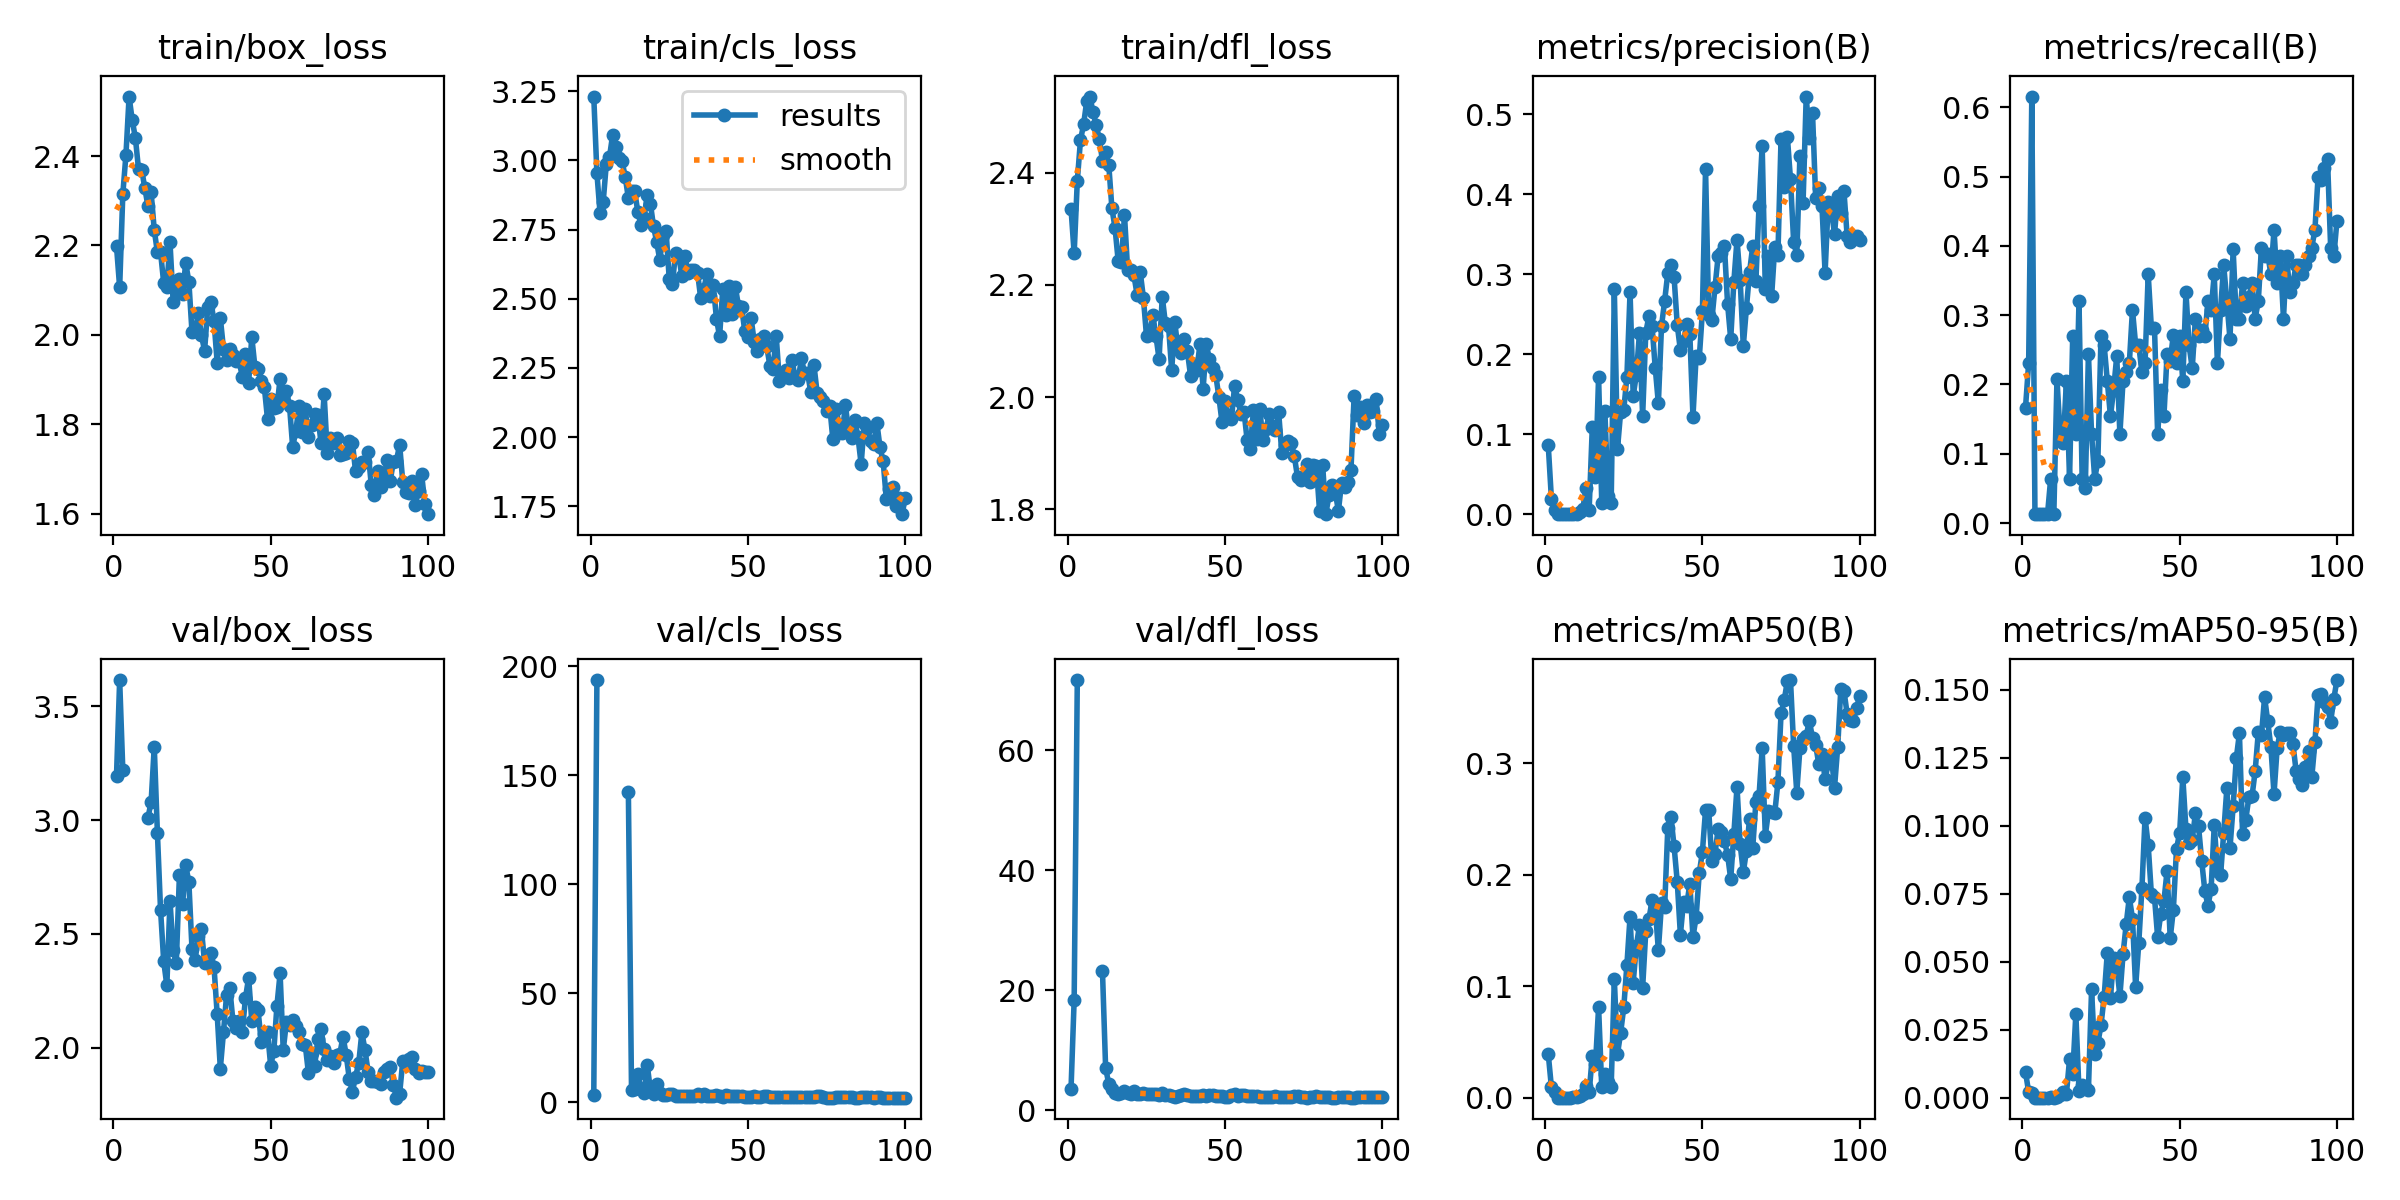
\includegraphics[width=0.6\linewidth]{assets/yolov8m_results.png}
    \caption{Hasil pelatihan YOLOv8m menunjukkan peningkatan lebih cepat pada precision dan recall dibanding YOLOv8s.}
    \label{fig:yolov8m_results}
\end{figure}

\begin{itemize}
    \item \textbf{train/box\_loss:} Menurun lebih lambat dibanding YOLOv8s tetapi mencapai nilai akhir yang lebih rendah.
    \item \textbf{train/cls\_loss:} Pola penurunan serupa, menunjukkan peningkatan akurasi klasifikasi.
    \item \textbf{train/obj\_loss:} Stabil setelah penurunan tajam di awal pelatihan.
    \item \textbf{metrics/precision(B):} Precision meningkat lebih cepat dibanding YOLOv8s, mengurangi kesalahan prediksi positif.
    \item \textbf{metrics/recall(B):} Recall meningkat signifikan, menunjukkan deteksi objek yang lebih baik.
    \item \textbf{metrics/mAP\_50(B):} mAP pada IoU 50 lebih tinggi dibanding YOLOv8s.
    \item \textbf{metrics/mAP\_50-95(B):} Rata-rata mAP menunjukkan performa lebih baik pada berbagai kondisi IoU.
    \item \textbf{val/loss (box, cls, obj):} Generalisasi validasi baik dengan pola penurunan loss yang konsisten.
\end{itemize}

\subsubsection{YOLOv8l}
YOLOv8l memberikan hasil terbaik di antara varian YOLOv8 dengan metrik performa tertinggi:

\begin{figure}[H]
    \centering
    \includegraphics[width=0.6\linewidth]{assets/yolov8l_results.png}
    \caption{Hasil pelatihan YOLOv8l menunjukkan metrik performa tertinggi dan generalisasi terbaik.}
    \label{fig:yolov8l_results}
\end{figure}

\begin{itemize}
    \item \textbf{train/box\_loss:} Menurun konsisten dengan nilai akhir terendah dibandingkan model lain.
    \item \textbf{train/cls\_loss:} Pola serupa tetapi dengan loss akhir yang lebih kecil dibanding YOLOv8m.
    \item \textbf{train/obj\_loss:} Stabil lebih awal dibanding model lainnya.
    \item \textbf{metrics/precision(B):} Precision tertinggi di antara semua model, menunjukkan sedikit kesalahan prediksi positif.
    \item \textbf{metrics/recall(B):} Recall juga tertinggi, menunjukkan jarang melewatkan deteksi objek.
    \item \textbf{metrics/mAP\_50(B):} mAP mencapai nilai tertinggi, menandakan performa optimal.
    \item \textbf{metrics/mAP\_50-95(B):} Performa rata-rata terbaik di berbagai kondisi IoU.
    \item \textbf{val/loss (box, cls, obj):} Loss validasi terendah, menunjukkan generalisasi yang sangat baik.
\end{itemize}

\subsubsection{YOLOv5s}

\begin{figure}[H]
    \centering
    \includegraphics[width=0.6\linewidth]{assets/yolov5s_results.png}
    \caption{Hasil pelatihan YOLOv5s menunjukkan performa yang stabil tetapi lebih rendah dibandingkan YOLOv8s.}
    \label{fig:yolov5s_results}
\end{figure}

\begin{itemize}
    \item \textbf{train/box\_loss:} Menurun lebih lambat dibanding YOLOv8s, dan loss akhirnya lebih tinggi.
    \item \textbf{train/cls\_loss:} Pola penurunan serupa dengan YOLOv8s, tetapi loss akhirnya lebih besar.
    \item \textbf{train/obj\_loss:} Menurun signifikan di awal, tetapi stabil di level yang lebih tinggi dibanding YOLOv8.
    \item \textbf{metrics/precision(B):} Precision meningkat tetapi lebih lambat dan lebih rendah dibanding YOLOv8.
    \item \textbf{metrics/recall(B):} Recall stabil tetapi lebih rendah dibanding YOLOv8.
    \item \textbf{metrics/mAP\_50(B):} mAP lebih rendah dari YOLOv8s, menunjukkan performa deteksi objek yang lebih rendah.
    \item \textbf{metrics/mAP\_50-95(B):} Performa rata-rata lebih rendah dibanding YOLOv8.
    \item \textbf{val/loss (box, cls, obj):} Loss validasi menunjukkan pola yang baik, tetapi generalisasi kurang dibanding YOLOv8.
\end{itemize}

\subsubsection{YOLOv5m}

\begin{figure}[H]
    \centering
    \includegraphics[width=0.6\linewidth]{assets/yolov5m_results.png}
    \caption{Hasil pelatihan YOLOv5m menunjukkan performa yang lebih rendah dibanding YOLOv8m.}
    \label{fig:yolov5m_results}
\end{figure}

\begin{itemize}
    \item \textbf{train/box\_loss:} Pola serupa dengan YOLOv8m, tetapi loss akhirnya lebih tinggi.
    \item \textbf{train/cls\_loss:} Menurun konsisten, tetapi tidak secepat YOLOv8m.
    \item \textbf{train/obj\_loss:} Stabil di level lebih tinggi dibanding YOLOv8m.
    \item \textbf{metrics/precision(B):} Precision lebih rendah dibanding YOLOv8m.
    \item \textbf{metrics/recall(B):} Recall meningkat, tetapi tidak secepat YOLOv8m.
    \item \textbf{metrics/mAP\_50(B):} mAP lebih rendah dibanding YOLOv8m.
    \item \textbf{metrics/mAP\_50-95(B):} Rata-rata mAP lebih rendah dibanding YOLOv8m.
    \item \textbf{val/loss (box, cls, obj):} Loss validasi lebih tinggi dibanding YOLOv8m.
\end{itemize}

\subsubsection{YOLOv5l}

\begin{figure}[H]
    \centering
    \includegraphics[width=0.6\linewidth]{assets/yolov5l_results.png}
    \caption{Hasil pelatihan YOLOv5l menunjukkan performa yang lebih rendah dibanding YOLOv8l.}
    \label{fig:yolov5l_results}
\end{figure}

\begin{itemize}
    \item \textbf{train/box\_loss:} Menurun lebih konsisten, tetapi masih lebih tinggi dibanding YOLOv8l.
    \item \textbf{train/cls\_loss:} Menurun baik, tetapi tidak secepat YOLOv8l.
    \item \textbf{train/obj\_loss:} Stabil di level yang lebih tinggi.
    \item \textbf{metrics/precision(B):} Precision lebih rendah dibanding YOLOv8l.
    \item \textbf{metrics/recall(B):} Recall lebih rendah dibanding YOLOv8l.
    \item \textbf{metrics/mAP\_50(B):} mAP lebih rendah dibanding YOLOv8l.
    \item \textbf{metrics/mAP\_50-95(B):} Performa rata-rata lebih rendah dibanding YOLOv8l.
    \item \textbf{val/loss (box, cls, obj):} Loss validasi lebih tinggi dibanding YOLOv8l.
\end{itemize}

\subsection{Diskusi Hasil}

Secara keseluruhan, hasil dari eksperimen ini menunjukkan bahwa varian YOLOv8 (YOLOv8s, YOLOv8m, dan YOLOv8l) memiliki performa yang lebih baik dibandingkan dengan varian YOLOv5 (YOLOv5s, YOLOv5m, dan YOLOv5l ) pada berbagai metrik evaluasi. YOLOv8l menunjukkan hasil terbaik di antara semua model, dengan penurunan loss yang konsisten dan metrik performa tertinggi seperti precision, recall, dan mAP. Hal ini menunjukkan bahwa model dengan parameter lebih besar, seperti YOLOv8l, mampu melakukan generalisasi yang lebih baik, meskipun memerlukan lebih banyak waktu pelatihan.

Sebaliknya, YOLOv5s, meskipun menunjukkan hasil yang stabil, memiliki performa yang lebih rendah dibandingkan YOLOv8s pada sebagian besar metrik, terutama pada nilai mAP dan precision. Hal ini mengindikasikan bahwa meskipun YOLOv5s lebih cepat dan lebih ringan, ia mungkin kurang efektif dalam mendeteksi objek yang lebih kompleks atau dalam kasus-kasus dengan tingkat kesulitan tinggi.

Selain itu, meskipun YOLOv8m menunjukkan peningkatan yang cepat pada precision dan recall, metrik performanya tidak sebaik YOLOv8l. Hal ini menunjukkan bahwa meskipun model dengan parameter sedang seperti YOLOv8m dapat memberikan hasil yang baik pada beberapa kasus, peningkatan ukuran model menjadi kunci untuk meningkatkan performa di seluruh metrik evaluasi.

Kesimpulannya, pemilihan model yang tepat harus disesuaikan dengan kebutuhan dan sumber daya yang tersedia. YOLOv8l menawarkan performa terbaik dalam hal deteksi objek, namun membutuhkan lebih banyak sumber daya dan waktu pelatihan. YOLOv8s dan YOLOv8m dapat menjadi alternatif yang lebih efisien dalam situasi dengan keterbatasan sumber daya atau waktu pelatihan yang lebih singkat, namun dengan kompromi pada hasil yang lebih rendah dibandingkan YOLOv8l.


% 5. Conclusion
\newpage
\section{Conclusion}

Penelitian ini bertujuan untuk meningkatkan keselamatan pejalan kaki di sekitar Kampus Unhas Tamalanrea dengan menyediakan dataset yang berisi gambar-gambar spot berbahaya yang dapat mengancam keselamatan pejalan kaki. Dataset ini mencakup berbagai kondisi infrastruktur yang tidak aman, seperti trotoar yang rusak, penghalang fisik, dan objek yang mengurangi ruang pejalan kaki. Melalui dataset ini, pihak kampus dapat mengidentifikasi titik-titik rawan dan merencanakan perbaikan yang lebih efektif.

Hasil pengujian model deteksi objek menggunakan YOLO menunjukkan bahwa model-model seperti YOLOv8s, YOLOv8m, dan YOLOv5s memberikan performa yang baik dalam mendeteksi objek berbahaya di area kampus. Model YOLOv8s dan YOLOv8m menunjukkan keseimbangan yang baik antara precision dan recall, sementara YOLOv5s unggul dalam hal akurasi dan recall. Meskipun model YOLOv8l menunjukkan hasil terbaik dalam hal precision, recall, dan mAP, semua model menunjukkan peningkatan performa yang signifikan seiring berjalannya waktu.

Secara keseluruhan, penelitian ini memberikan kontribusi yang penting dalam upaya meningkatkan keselamatan pejalan kaki di kampus. Dataset yang dihasilkan dapat digunakan untuk analisis lebih lanjut dan sebagai dasar pengambilan keputusan berbasis data dalam memperbaiki infrastruktur kampus. Dengan demikian, dataset ini dapat mendukung perancangan kebijakan keselamatan pejalan kaki yang lebih baik serta mempercepat program perbaikan infrastruktur yang lebih tepat sasaran.



\newpage

\bibliographystyle{plain}
\begin{thebibliography}{3}

\bibitem{zhang2013} Zhang, Y., Gawade, M., Lin, P. S., \& McPherson, T. (2013). Educational campaign for improving pedestrian safety: a university campus study. \textit{Procedia-Social and Behavioral Sciences}, 96, 2756-2766.

\bibitem{rizvina2023} Rizvina, V., Sari, L. H., \& Djamaluddin, M. (2023). Analisis Jalur Pedestrian Melalui Konsep Walkability (Studi Kasus: Jalan Diponegoro, Pasar Aceh). \textit{Jurnal Ilmiah Mahasiswa Arsitektur dan Perencanaan}, 7(1), 108-118.

\bibitem{widianti2017} Widianti, N. T., \& Rohmawati, T. (2017). Persepsi Pejalan Kaki Terhadap Kondisi Fisik Trotoar Jalan Dipatiukur. \textit{Prosiding SAINTIKS FTIK UNIKOM}, 2.

\end{thebibliography}


\end{document}